\documentclass{llncs}
\usepackage[utf8]{inputenc}
\usepackage{amsmath}
\usepackage{graphicx}
\usepackage{booktabs}
\usepackage{float}
\usepackage{placeins}
\usepackage{url}

\begin{document}

\title{Authenticated Image Encryption with Frequency-Domain Convolution Whitening and a Password-Derived Key}

\author{M.C. Zuriel L\'opez Sosa \and Dra. B\'arbara Emma S\'anchez Rinza \and
Dr. Carlos Ignacio Robledo S\'anchez}
\institute{Benemerita Universidad Autonoma de Puebla\\
\email{zuriel.lopezs@correo.buap.mx, brinza@fcfm.buap.mx, crobledo@fcfm.buap.mx}}

\maketitle

\begin{center}
Source code available at: \url{https://github.com/zuriells/cifrado-imagenes-fft}
\end{center}

\begin{abstract}
Image encryption is essential for secure digital communication and the
protection of visual data. This paper presents a method that combines a
frequency-domain \emph{whitening} transform with \textbf{authenticated
encryption}. The whitening transform relies on the convolution property of
the Fourier Transform (FT): the original image and a password-derived key
are transformed into the frequency domain and multiplied element-wise,
producing a decorrelated representation with no visual resemblance to the
original. Since this convolution is a \emph{linear} operation and, by
itself, does not constitute a secure cipher, the whitened representation is
passed through a \textbf{confusion-diffusion} stage (key-dependent
permutation and nonlinear diffusion over several rounds) that breaks this
linearity and gives the image cipher resistance to plaintext attacks.
Finally, confidentiality and integrity are delegated to
\textbf{ChaCha20-Poly1305} (RFC 8439): the result is sealed with a key
derived from the password using PBKDF2-HMAC-SHA256 and SHAKE-256. The result is stored as a
16-bit-per-channel PNG with the nonce, authentication tag, salt, and
normalization metadata embedded in the file, removing the need for an
external key file. To evaluate the method, over 18 images of different
resolution and content from the USC-SIPI database, statistical analyses
(histograms, entropy, pixel correlation), a comparison with AES-256, a
performance evaluation, diffusion tests (NPCR, UACI, and key sensitivity), and
security tests against incorrect-password, Gaussian noise, and resizing
manipulations were performed. The results show that the encrypted image
exhibits near-maximal entropy ($\approx 8$ bits/pixel), a uniform histogram,
and near-ideal NPCR and UACI values, that decryption with the correct
password recovers the original image \textbf{exactly} (infinite PSNR), and
that \textbf{any}
alteration of the encrypted file or the password is detected and rejected by
the authentication tag, so that the scheme is non-malleable.

\keywords{Image encryption, authenticated encryption, ChaCha20-Poly1305,
confusion-diffusion, NPCR, UACI, Fourier Transform, key derivation, PBKDF2,
SHAKE-256, integrity, cryptographic analysis.}
\end{abstract}

\section{Introduction}

In the digital age, information security is a priority, particularly
regarding the protection of images, which often contain sensitive data.
Digital images, due to their visual nature, present an additional challenge
for traditional spatial-domain encryption methods. Frequency-domain
processing techniques, such as those based on the Fourier Transform (FT),
have gained attention for their ability to effectively decorrelate and
conceal data patterns \cite{refregier,unnikrishnan}. Existing alternatives
include random phase encoding schemes in the optical domain \cite{javidi}
and chaos-based schemes \cite{chaos1,chaos2}, which pursue similar
randomization goals through nonlinear spatial-domain dynamics.

However, a frequently underestimated point is that linear combination in the
frequency domain --- multiplying the FT of the image by that of a key --- is
itself a \emph{linear} cipher and therefore insecure: given a single
(image, ciphertext) pair, an attacker can solve for the key in the frequency
domain, $\mathcal{F}(g) = \mathcal{F}(f*g)/\mathcal{F}(f)$, and decrypt any
other image protected with the same key. This is precisely the weakness that
breaks linear optical double random phase encoding schemes under known- and
chosen-plaintext attacks \cite{peng,frauel}. Consequently, a scheme that
rests its confidentiality solely on this operation cannot satisfy the formal
security notions, which require that an attacker without the key be unable to
distinguish the ciphertext from random noise or to alter it undetected
\cite{bellare,aead}.

This work adopts a layered design that resolves this limitation. First,
frequency-domain convolution is retained as a \textbf{reversible whitening
transform} --- useful for decorrelating the image and analyzing its
statistical properties. Second, a \textbf{confusion-diffusion} stage, in the
spirit of Fridrich's architecture \cite{fridrich} (position permutation and
nonlinear diffusion over several rounds), breaks the linearity of the
whitening and gives the image cipher full diffusion and resistance to known-
and chosen-plaintext attacks, evidenced by near-ideal NPCR and UACI values.
Third, confidentiality and integrity are delegated entirely to a standard
\textbf{authenticated cipher}, ChaCha20-Poly1305 \cite{rfc8439}. The key is
derived from a \textbf{password} using standard
cryptographic functions (following Kerckhoffs's principle \cite{kerckhoffs}),
so that only the encrypted file and the password are needed to recover the
original image.

The aim of this paper is to present and evaluate this method, examining its
effectiveness and security. Evaluation is conducted through statistical
tests (histogram comparison, entropy, and PSNR) and integrity tests against
manipulations of the encrypted file.

The structure of this article is as follows: Section 2 describes the
proposed algorithm, detailing the whitening transform, the key derivation,
and the encryption and decryption processes. Section 3 presents the tests
performed and the analysis of results. Finally, Section 4 concludes with a
discussion of the findings.

\section{Methodology}

The method consists of three clearly separated layers: a \textbf{whitening
transform} in the frequency domain (reversible, but which does \emph{not}
provide security by itself), a \textbf{confusion-diffusion} stage (which
breaks the linearity and diffuses any change across the whole array), and an
\textbf{authenticated encryption} layer (which provides confidentiality and
integrity with standard backing). This separation is deliberate: the
security guarantees do not depend on the linear operation, but on a
nonlinear stage with full diffusion and on a standardized, widely analyzed
cryptographic primitive.

\subsection{Whitening transform by convolution}

The whitening transform is based on the \textbf{Fourier Transform convolution
property}, which states that the Fourier transform of the convolution of two
functions equals the product of their respective Fourier transforms:
\[
\mathcal{F}(f * g) = \mathcal{F}(f) \cdot \mathcal{F}(g)
\]
Isolating the convolution term and applying the Inverse Fourier Transform
($\mathcal{F}^{-1}$) on both sides gives:
\[
f * g = \mathcal{F}^{-1}\left(\mathcal{F}(f) \cdot \mathcal{F}(g)\right)
\]
This implies that convolution in the spatial domain can be computed
indirectly through multiplication in the frequency domain, followed by the
Inverse Transform. In practice, both transforms are computed using the Fast
Fourier Transform (FFT) algorithm \cite{cooley}, which reduces the
computational complexity from $O(N^2)$ to $O(N\log N)$.

Throughout this article, $f$ denotes the \textbf{original image} and $g$
denotes the \textbf{key image}. The whitened representation is the
convolution $f * g$, computed in the frequency domain as described above. To
invert the whitening, it suffices to solve for $f$ by dividing in the
frequency domain by $\mathcal{F}(g)$ instead of multiplying:
\[
f = \mathcal{F}^{-1}\left(\frac{\mathcal{F}(f * g)}{\mathcal{F}(g)}\right)
\]
Since the images used are in RGB format, all operations are performed
independently on each of the three color channels (Red, Green, and Blue).

It must be emphasized that this transform is \emph{linear} and is therefore
\textbf{not} used as a confidentiality mechanism: it serves only to
decorrelate the image before encrypting it. Security is provided by the
confusion-diffusion stage (Section~2.3) and the authenticated cipher
(Section~2.4).

\subsection{Deriving the key from a password}

Instead of requiring an external key file, all cryptographic material is
generated from a password. This design follows Kerckhoffs's principle
\cite{kerckhoffs}: security relies solely on the secrecy of the password and
not on that of the algorithm. The derivation uses password-based key
derivation functions \cite{nist800132,scrypt}:

\begin{enumerate}
  \item A random 16-byte salt and a random 12-byte nonce are generated at
    encryption time.
  \item The password and salt are processed with \textbf{PBKDF2-HMAC-SHA256}
    \cite{pbkdf2} using 310{,}000 iterations, producing a \textbf{master
    secret} of 32 bytes. This secret is the ChaCha20-Poly1305 key.
  \item From the master secret, the key image $g$ is generated at exactly
    the image's size: \textbf{SHAKE-256} (an extendable-output function from
    the SHA-3 family \cite{sha3}), applied to the secret with a domain
    separator, is expanded to $\text{height}\times\text{width}\times 3$
    bytes. The separator avoids reusing the master secret directly as the
    whitening seed.
\end{enumerate}

\textbf{Key space.} The master secret is 256 bits, so the derived-key space
is $2^{256}$, well above the $2^{128}$ threshold considered brute-force
resistant. The 128-bit salt ensures that the same password produces different
keys on each encryption, and the 96-bit nonce guarantees the uniqueness
required by ChaCha20-Poly1305. Resistance with respect to the password itself
is determined by its entropy and reinforced by the 310{,}000 PBKDF2
iterations, which make each guessing attempt costly.

\subsection{Confusion-diffusion}

So that the method has its own robustness as an image cipher and does not
rest its security solely on the authenticated envelope, the whitened
representation is passed through a confusion-diffusion stage, in the spirit
of Fridrich's classical architecture \cite{fridrich}. $R=3$ rounds are
applied; in each round, over the byte array:

\begin{enumerate}
  \item \textbf{Nonlinear diffusion}: a pseudorandom stream (keystream) is
    added modulo 256 and an accumulated XOR chaining is applied, so that
    each output byte depends on all previous ones. The combination of modular
    addition and XOR introduces nonlinearity and a strong avalanche effect.
  \item \textbf{Confusion}: byte positions are permuted using a key-dependent
    permutation.
\end{enumerate}

The keystream, the permutation, and the initialization vector of each round
are derived reproducibly with SHAKE-256 from $(\text{secret},
\text{nonce}, \text{round})$, so that decryption regenerates exactly the
same material and reverses the rounds in inverse order. By mixing modular
addition, XOR, and permutation, the overall transform ceases to be linear:
the known-plaintext attack $\mathcal{F}(g)=\mathcal{F}(f*g)/\mathcal{F}(f)$
no longer applies. The effectiveness of this stage is quantified in
Section~3.3 through NPCR, UACI, and key sensitivity.

\subsection{Encryption process}

\begin{enumerate}
  \item \textbf{Inputs}: the original image $f$ and a password.
  \item \textbf{Derivation}: the master secret and the key image $g$ are
    obtained as in Section~2.2.
  \item \textbf{Whitening}: $f*g$ is computed channel-wise in the frequency
    domain (Section~2.1). Since the convolution result has a much larger
    value range than a conventional image, per-channel Min-Max normalization
    to a 16-bit range ($[0,65535]$) is applied; the per-channel minimum and
    maximum are kept as metadata so the whitening can be inverted without
    loss.
  \item \textbf{Confusion-diffusion}: the whitened representation, serialized
    to bytes, is transformed with the $R=3$ rounds described in Section~2.3.
  \item \textbf{Authenticated sealing}: the result is encrypted with
    \textbf{ChaCha20-Poly1305} \cite{rfc8439}, using the master secret as the
    key and the generated nonce. The salt, nonce, iteration count, and
    normalization ranges are passed as \emph{authenticated associated data}
    (AAD), so they are also protected against tampering even though they
    travel in the clear.
  \item \textbf{Storage}: the encrypted output (the same length as the
    input) is reinterpreted as a 16-bit-per-channel image and stored as a
    PNG. The nonce, the authentication tag (Poly1305), the salt, and the
    ranges are embedded as metadata in a JSON-encoded \texttt{tEXt} chunk, so
    the resulting file is self-contained. This file is the \textbf{encrypted
    image}.
\end{enumerate}

\subsection{Decryption process}

\begin{enumerate}
  \item \textbf{Inputs}: the encrypted image and the password.
  \item \textbf{Reading metadata}: the salt, nonce, authentication tag,
    iteration count, and per-channel min/max ranges are read from the file.
  \item \textbf{Re-derivation}: the process from Section~2.2 is repeated with
    the same salt, regenerating the master secret and the key image $g$.
  \item \textbf{Verification and decryption}: ChaCha20-Poly1305 verifies the
    authentication tag before decrypting. \textbf{If the password is
    incorrect or the file was altered, verification fails and the process is
    aborted without producing any image.}
  \item \textbf{Inverting the confusion-diffusion}: only when authentication
    succeeds are the $R=3$ rounds of Section~2.3 undone in inverse order,
    recovering the whitened representation.
  \item \textbf{Inverting the whitening}: the 16-bit normalization is
    reversed and $f$ recovered by dividing in the frequency domain:
    \[
    f \approx \mathcal{F}^{-1}\left(\frac{\mathcal{F}(f * g)}{\mathcal{F}(g) + \epsilon}\right)
    \]
    with $\epsilon = 1\times10^{-10}$ to avoid division by zero.
  \item \textbf{Rounding and clipping}: the result is rounded and clipped to
    the valid $[0,255]$ range to obtain the final 8-bit image.
\end{enumerate}

\section{Analysis and Performance Evaluation}

This section presents the analysis and evaluation of the proposed method. To
verify that the observed behavior is not dependent on a single image, the
statistical and security evaluation was carried out on a diverse subset of
\textbf{18 images} from the USC-SIPI Image Database \cite{sipi} --- of varied
content (natural, aerial, and texture, in color and grayscale) and at
resolutions of $256\times256$, $512\times512$, and $1024\times1024$ --- and
the results are reported in aggregate (mean $\pm$ standard deviation). For the
illustrative figures and the performance evaluation, a $3024\times4032$-pixel
photograph and a $2250\times2250$ aerial image are additionally used. The
evaluation comprises: visual inspection, statistical analysis (histogram,
entropy, correlation), diffusion (NPCR, UACI, key sensitivity), comparison
with a standard cipher, integrity testing, and performance evaluation.

\subsection{Visual inspection}

\begin{figure}[htbp]
  \centering
  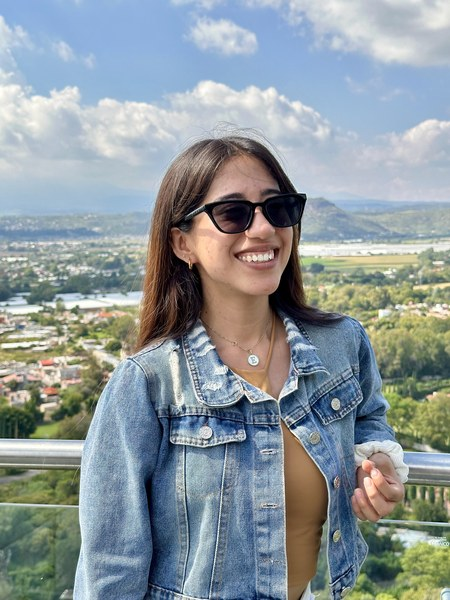
\includegraphics[width=0.3\textwidth]{eval_original.jpg}
  \hfill
  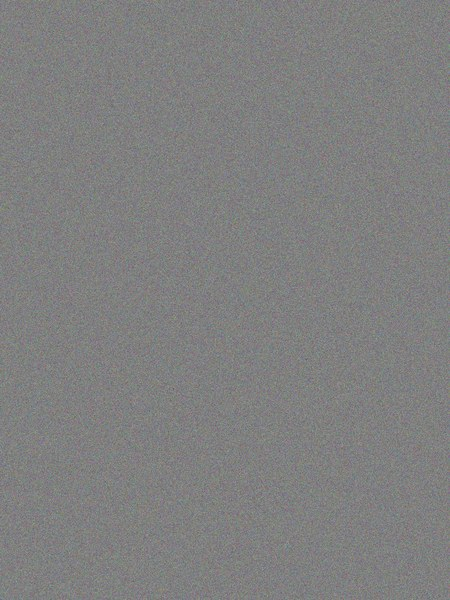
\includegraphics[width=0.3\textwidth]{eval_encrypted.jpg}
  \hfill
  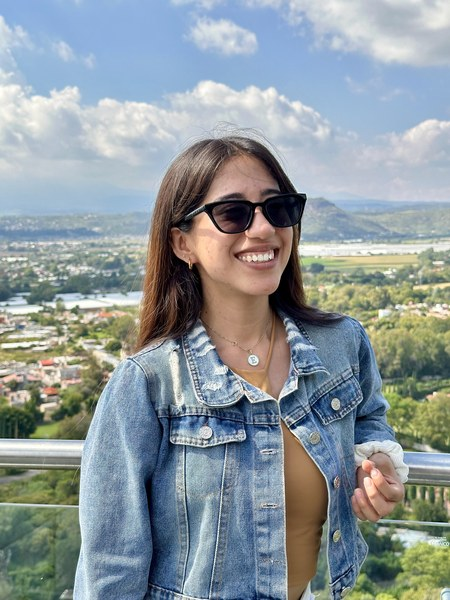
\includegraphics[width=0.3\textwidth]{eval_correct.jpg}
  \caption{Left to right: original image $f$, encrypted image (8-bit preview
  of the actual 16-bit data), and decrypted image (recovery of $f$) obtained
  by decrypting with the correct password.}
\end{figure}
\FloatBarrier

The encrypted image shows no recognizable trace of $f$'s content, while the
decrypted image is, as quantified in Section~3.2, identical to $f$.

\subsection{Statistical analysis}

\subsubsection{Histogram analysis.}
Intensity histograms are a standard tool for analyzing the pixel-value
distribution of an image \cite{gonzalez}. Histograms of $f$ and of the
encrypted image were computed for each color channel (Fig.~2). The original
image's histogram shows pronounced peaks associated with regions of uniform
color (sky, skin, clothing). The encrypted image's histogram, in contrast, is
\textbf{essentially uniform}: the peaked structure of the original disappears
entirely. This result is consistent with the output of an authenticated
cipher, which is computationally indistinguishable from a uniform random
sequence. (Note that the intermediate \emph{whitened} representation, before
sealing, exhibits a Gaussian shape by the central limit theorem applied to
convolution; the uniform histogram in Fig.~2 corresponds to the final,
encrypted output.)

\begin{figure}[htbp]
  \centering
  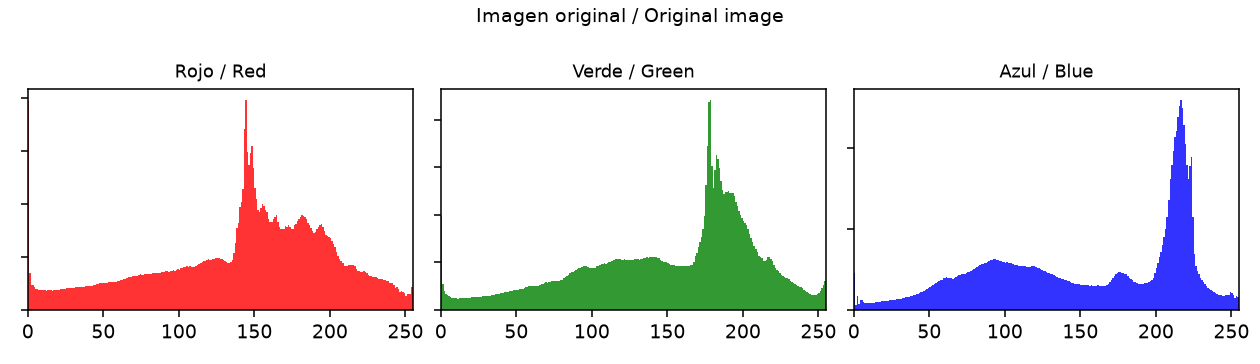
\includegraphics[width=0.9\textwidth]{hist_original.png}\\[4pt]
  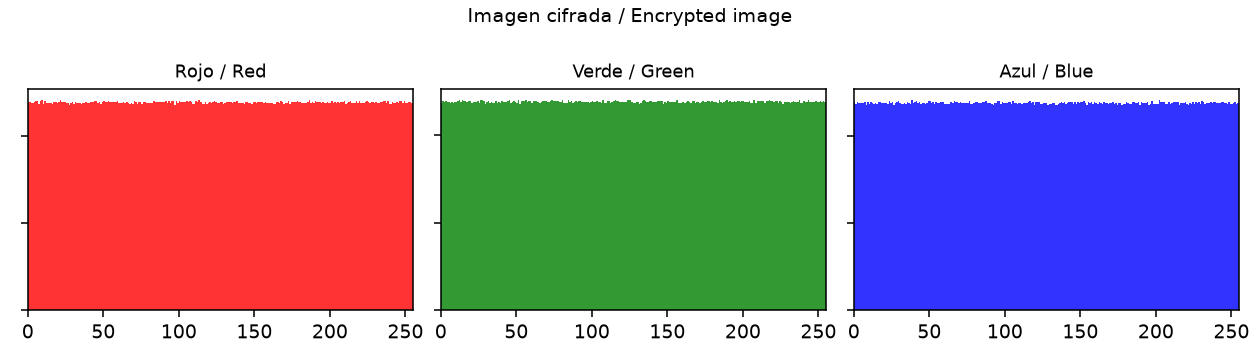
\includegraphics[width=0.9\textwidth]{hist_encrypted.png}
  \caption{Per-channel (R, G, B) histograms of the original image (top) and
  the encrypted image (bottom).}
\end{figure}
\FloatBarrier

\subsubsection{Entropy analysis.}
Shannon entropy \cite{shannon} was computed over the \emph{8-bit
visualization} of the encrypted image (the high byte of the 16-bit data),
averaged over the three channels. Across the 18-image set, the mean entropy
of the encrypted image is $7.9990 \pm 0.0009$ bits/pixel (range
$[7.9970, 7.9998]$), versus $7.0837 \pm 0.4082$ for the originals. This value
is practically equal to the theoretical maximum of $8$ bits/pixel and matches
that produced by a standard cipher on the same images (AES-256-CTR: $7.9990$;
Section~3.4). It should be emphasized that this near-maximal entropy stems
from the output being that of an authenticated cipher (indistinguishable from
a uniform sequence); a plain 8-bit normalization of the whitening, in
contrast, concentrates the values into a bell shape and yields substantially
lower entropy, and should therefore \emph{not} be used as evidence of
randomness.

\subsubsection{PSNR evaluation.}
The Peak Signal-to-Noise Ratio (PSNR) \cite{psnr} between $f$ and the image
recovered by decrypting with the correct password was computed. The result
obtained was:
\[
\text{MSE} = 0.0 \qquad \text{PSNR} = \infty
\]
That is, the recovered image is \textbf{bit-for-bit identical} to the
original. Recovery was exact (MSE $=0$, infinite PSNR) for all 18 images in
the set, without exception. This confirms that, by using 16 bits per channel
with the normalization ranges stored as exact metadata, the full encryption
and decryption process introduces no information loss whatsoever.

\subsubsection{Adjacent-pixel correlation.}
In a natural image, neighboring pixels are strongly correlated; a good cipher
must reduce this correlation to practically zero \cite{gonzalez}. The
correlation coefficient between adjacent pixel pairs was measured in the
horizontal (H), vertical (V), and diagonal (D) directions, averaged over the
channels. Table~1 shows the aggregate values over the 18 images: correlation
drops from $\approx 0.88$ in the originals to $\approx 0.001$ in the encrypted
images, in all three directions. Moreover, the global correlation between the
original and the encrypted image (plaintext--ciphertext) is
$0.0012 \pm 0.0012$, i.e., the output retains no linear relationship with the
input. Fig.~3 illustrates this effect with adjacent-pixel scatter plots.

\begin{table}[htbp]
  \centering
  \caption{Adjacent-pixel correlation coefficient (mean $\pm$ standard
  deviation over 18 images).}
  \begin{tabular}{@{}lcc@{}}
    \toprule
    \textbf{Direction} & \textbf{Original} & \textbf{Encrypted} \\
    \midrule
    Horizontal & $0.9038 \pm 0.0817$ & $-0.0014 \pm 0.0065$ \\
    Vertical   & $0.8979 \pm 0.0772$ & $\phantom{-}0.0007 \pm 0.0103$ \\
    Diagonal   & $0.8395 \pm 0.1330$ & $-0.0005 \pm 0.0070$ \\
    \bottomrule
  \end{tabular}
\end{table}
\FloatBarrier

\begin{figure}[htbp]
  \centering
  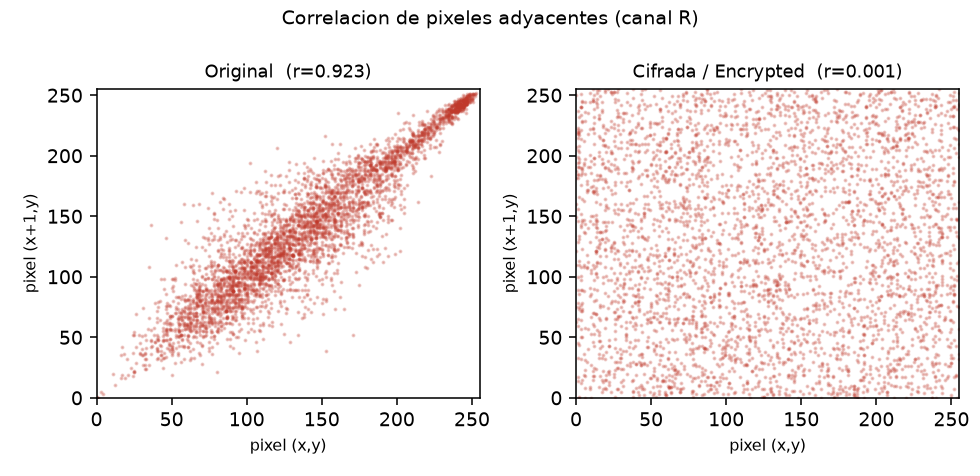
\includegraphics[width=0.85\textwidth]{corr_scatter.png}
  \caption{Adjacent-pixel scatter (R channel, horizontal direction) for a
  representative image: original (left) and encrypted (right). The strong
  diagonal of the original disappears entirely after encryption.}
\end{figure}
\FloatBarrier

\subsection{Diffusion: NPCR and UACI}

To evaluate the diffusion of the image cipher (the whitening plus the
confusion-diffusion stage, before the authenticated envelope), the standard
NPCR (Number of Pixels Change Rate) and UACI (Unified Average Changing
Intensity) tests \cite{npcr} were used, which measure how the encrypted
output changes when a single input pixel is modified. For each image, two
versions identical except for a single pixel were encrypted with the same
key, and the core outputs were compared. Key sensitivity was also measured,
by encrypting each image with two keys differing in a single bit. The
aggregate results over the 18 images (Table~2) are practically identical to
the ideal values, confirming full diffusion: a minimal change in the input,
or in the key, alters almost the entire encrypted output.

\begin{table}[htbp]
  \centering
  \caption{Diffusion metrics of the cipher core (mean $\pm$ standard
  deviation over 18 images).}
  \begin{tabular}{@{}lcc@{}}
    \toprule
    \textbf{Metric} & \textbf{Obtained} & \textbf{Ideal} \\
    \midrule
    NPCR            & $99.6105 \pm 0.0035$\% & $99.6094$\% \\
    UACI            & $33.4658 \pm 0.0173$\% & $33.4635$\% \\
    Key sensitivity & $99.6087 \pm 0.0042$\% & $\approx 99.61$\% \\
    \bottomrule
  \end{tabular}
\end{table}
\FloatBarrier

\subsection{Comparison with a standard cipher}

To objectively assess the method, its statistical metrics were compared with
those of a widely established cipher, AES-256 in CTR mode \cite{aes}, applied
to the same 18 images (Table~4). In both cases the entropy is practically
maximal and the adjacent-pixel correlation is indistinguishable from zero,
indicating that the output of the proposed method is statistically equivalent
to that of a standard cipher. Regarding NPCR and UACI, the proposed core
attains near-ideal values, comparable to those reported by chaotic-map image
encryption schemes \cite{chaos1,chaos2}. Note that NPCR and UACI measure
diffusion with respect to the \emph{plaintext}, characteristic of image
ciphers, and are not applicable to a stream cipher such as AES-CTR (whose
security comes from nonce randomization, not per-pixel diffusion).

\begin{table}[htbp]
  \centering
  \caption{Comparison of statistical metrics (mean over 18 images) between the
  proposed method and AES-256-CTR.}
  \begin{tabular}{@{}lccc@{}}
    \toprule
    \textbf{Metric} & \textbf{Proposed} & \textbf{AES-256-CTR} & \textbf{Ideal} \\
    \midrule
    Encrypted entropy         & $7.9990$  & $7.9990$  & $8$ \\
    $|r|$ adjacent (mean)      & $0.0065$  & $0.0073$  & $0$ \\
    $|r|$ plaintext--ciphertext & $0.0012$  & ---       & $0$ \\
    NPCR                       & $99.61$\% & n/a       & $99.61$\% \\
    UACI                       & $33.47$\% & n/a       & $33.46$\% \\
    \bottomrule
  \end{tabular}
\end{table}
\FloatBarrier

\subsection{Integrity and authentication}

Unlike a pure linear cipher, in which tampering with the file yields a
degraded but potentially still useful image for an attacker, an authenticated
cipher is \textbf{non-malleable}: any alteration of the password or the
encrypted file invalidates the Poly1305 tag, and decryption is
\textbf{rejected}. Three families of manipulations were evaluated ---
including resizing with symmetric factors ($\pm1\%$, $\pm5\%$, $\pm10\%$) ---
plus a single-bit flip; the results are summarized in Table~3. It should be
clarified that the inability to decrypt a manipulated image is \textbf{not}
interpreted here as heuristic ``tamper detection,'' but stems from an
explicit authentication mechanism (the Poly1305 tag), which is what
legitimizes the integrity claim.

\begin{table}[htbp]
  \centering
  \caption{Outcome of the decryption attempt under different manipulations of
  the encrypted file or the password (identical across all 18 images).}
  \begin{tabular}{@{}lc@{}}
    \toprule
    \textbf{Attack / manipulation} & \textbf{Outcome} \\
    \midrule
    Incorrect password                        & Rejected \\
    Gaussian noise ($\sigma \approx 32.8$)     & Rejected \\
    Gaussian noise ($\sigma \approx 163.8$)    & Rejected \\
    Gaussian noise ($\sigma \approx 327.7$)    & Rejected \\
    Resizing $-1\%, -5\%, -10\%$               & Rejected \\
    Resizing $+1\%, +5\%, +10\%$               & Rejected \\
    Single-bit flip                            & Rejected \\
    \bottomrule
  \end{tabular}
\end{table}
\FloatBarrier

In all cases, including the smallest possible perturbation --- a single-bit
change --- ChaCha20-Poly1305 detected the alteration and rejected the
decryption. This behavior is qualitatively superior to that of an
unauthenticated cipher: the system not only protects confidentiality but
\textbf{guarantees the integrity and authenticity} of the encrypted file, so
that no manipulation --- however small --- can go unnoticed or be exploited
to obtain a partial reconstruction of the image.

\subsection{Performance evaluation}

Encryption and decryption times were measured for images of different sizes,
from $256\times256$ up to $3024\times4032$ pixels (Table~5). Throughput stays
around $6$--$9$ MB/s. It is worth noting that the PBKDF2 key derivation
(310{,}000 iterations) is a fixed per-operation cost, deliberately chosen to
hinder brute force on the password; it therefore dominates the time for the
smallest images. The remaining time grows approximately linearly with the
number of pixels (Fig.~4), consistent with the $O(N\log N)$ cost of the FFT
and $O(N)$ of the confusion-diffusion. Memory consumption also scales linearly
with image size; its peak (dominated by the confusion-diffusion permutations)
was about $4.5$ GB for the $12$-megapixel image, which constitutes a
limitation to be optimized in future work (for example, by block-wise
processing).

\begin{table}[htbp]
  \centering
  \caption{Encryption/decryption times and throughput by image size.}
  \begin{tabular}{@{}lcccc@{}}
    \toprule
    \textbf{Size} & \textbf{MP} & \textbf{Encrypt (s)} & \textbf{Decrypt (s)} & \textbf{Throughput (MB/s)} \\
    \midrule
    $256\times256$   & $0.07$  & $0.05$ & $0.04$ & $4.2$--$5.3$ \\
    $512\times512$   & $0.26$  & $0.09$ & $0.09$ & $9.0$ \\
    $1024\times1024$ & $1.05$  & $0.33$ & $0.40$ & $7.9$--$9.5$ \\
    $2250\times2250$ & $5.06$  & $1.92$ & $2.25$ & $6.7$--$7.9$ \\
    $3024\times4032$ & $12.19$ & $5.41$ & $6.13$ & $6.0$--$6.8$ \\
    \bottomrule
  \end{tabular}
\end{table}
\FloatBarrier

\begin{figure}[htbp]
  \centering
  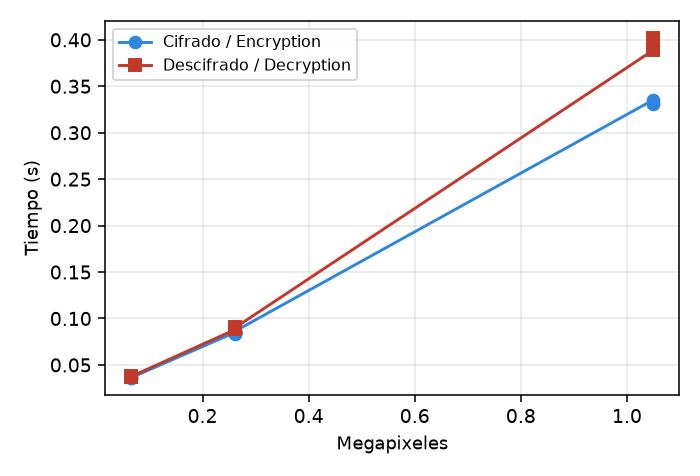
\includegraphics[width=0.6\textwidth]{perf_time.png}
  \caption{Encryption and decryption times as a function of the number of
  megapixels.}
\end{figure}
\FloatBarrier

\section{Conclusions}

The analysis demonstrates that the proposed method effectively transforms an
image's content into an encrypted representation with a randomized
appearance, near-maximal entropy ($\approx 8$ bits/pixel), and a uniform
histogram, computationally indistinguishable from noise. The central point of
the design is to recognize that linear convolution in the frequency domain,
although useful for decorrelating the image, is insecure on its own ---
vulnerable to known- and chosen-plaintext attacks \cite{peng,frauel} --- and
therefore to add a confusion-diffusion stage that breaks this linearity and
achieves full diffusion (near-ideal NPCR $99.61\%$ and UACI $33.46\%$, with
$99.61\%$ key sensitivity), and to delegate confidentiality and integrity to
a standard authenticated cipher (ChaCha20-Poly1305).

The evaluation over a set of 18 images of different resolution and content
confirms that these results are not image-dependent: entropy
$7.9990 \pm 0.0009$, adjacent-pixel correlation reduced from $\approx 0.88$ to
$\approx 0.001$, and plaintext--ciphertext correlation of $\approx 0.001$,
values statistically equivalent to those of a standard cipher (AES-256).
Decryption with the correct password recovers the original image
\textbf{exactly} (infinite PSNR) in all of them, thanks to the
16-bit-per-channel storage
with precise normalization ranges. The integrity tests show that \textbf{any}
alteration of the password or the encrypted file --- noise, resizing, or even
a single-bit change --- is detected and rejected by the authentication tag, a
non-malleability property especially valuable for detecting and preventing
unauthorized tampering. Overall, the scheme provides confidentiality,
integrity, and authenticity with security backed by standard primitives, while
also removing the need to distribute a separate key file, making it practical
for secure image transmission.

\begin{thebibliography}{23}
\bibitem{refregier} Refregier, P., Javidi, B.: Optical image encryption
  based on input plane and Fourier plane random encoding. Optics Letters
  20(7), 767--769 (1995).
\bibitem{unnikrishnan} Unnikrishnan, G., Joseph, J., Singh, K.: Optical
  encryption system that uses phase conjugation in a photorefractive
  crystal. Applied Optics 37(35), 8181--8186 (1998).
\bibitem{javidi} Javidi, B., Zhang, G., Li, J.: Experimental demonstration of
  the random phase encoding technique for image encryption and security
  verification. Optical Engineering 35(9), 2506--2512 (1996).
\bibitem{chaos1} Chen, G., Mao, Y., Chui, C.K.: A symmetric image encryption
  scheme based on 3D chaotic cat maps. Chaos, Solitons \& Fractals 21(3),
  749--761 (2004).
\bibitem{chaos2} Zhou, Y., Bao, L., Chen, C.L.P.: A new 1D chaotic system for
  image encryption. Signal Processing 97, 172--182 (2014).
\bibitem{cooley} Cooley, J.W., Tukey, J.W.: An algorithm for the machine
  calculation of complex Fourier series. Mathematics of Computation 19(90),
  297--301 (1965).
\bibitem{peng} Peng, X., Zhang, P., Wei, H., Yu, B.: Known-plaintext attack
  on optical encryption based on double random phase keys. Optics Letters
  31(8), 1044--1046 (2006).
\bibitem{frauel} Frauel, Y., Castro, A., Naughton, T.J., Javidi, B.:
  Resistance of the double random phase encryption against various attacks.
  Optics Express 15(16), 10253--10265 (2007).
\bibitem{kerckhoffs} Kerckhoffs, A.: La cryptographie militaire. Journal des
  sciences militaires 9, 5--38 (1883).
\bibitem{pbkdf2} Moriarty, K., Kaliski, B., Rusch, A.: PKCS \#5: Password-Based
  Cryptography Specification, Version 2.1. RFC 8018 (2017).
\bibitem{nist800132} Turan, M.S., Barker, E., Burr, W., Chen, L.:
  Recommendation for Password-Based Key Derivation, Part 1: Storage
  Applications. NIST Special Publication 800-132 (2010).
\bibitem{scrypt} Percival, C.: Stronger key derivation via sequential
  memory-hard functions. In: BSDCan 2009 (2009).
\bibitem{sha3} National Institute of Standards and Technology: SHA-3 Standard:
  Permutation-Based Hash and Extendable-Output Functions. FIPS PUB 202 (2015).
\bibitem{rfc8439} Nir, Y., Langley, A.: ChaCha20 and Poly1305 for IETF
  Protocols. RFC 8439 (2018).
\bibitem{aead} Bellare, M., Namprempre, C.: Authenticated encryption:
  Relations among notions and analysis of the generic composition paradigm.
  In: ASIACRYPT 2000, LNCS 1976, pp. 531--545 (2000).
\bibitem{fridrich} Fridrich, J.: Symmetric ciphers based on two-dimensional
  chaotic maps. International Journal of Bifurcation and Chaos 8(6),
  1259--1284 (1998).
\bibitem{npcr} Wu, Y., Noonan, J.P., Agaian, S.: NPCR and UACI randomness
  tests for image encryption. Cyber Journals: Journal of Selected Areas in
  Telecommunications, 31--38 (2011).
\bibitem{aes} National Institute of Standards and Technology: Advanced
  Encryption Standard (AES). FIPS PUB 197 (2001).
\bibitem{sipi} University of Southern California, Signal and Image Processing
  Institute: The USC-SIPI Image Database. \url{https://sipi.usc.edu/database}.
\bibitem{shannon} Shannon, C.E.: A mathematical theory of communication. The
  Bell System Technical Journal 27(3), 379--423 (1948).
\bibitem{gonzalez} Gonzalez, R.C., Woods, R.E.: Digital Image Processing,
  4th ed. Pearson (2018).
\bibitem{psnr} Hore, A., Ziou, D.: Image quality metrics: PSNR vs. SSIM. In:
  20th International Conference on Pattern Recognition (ICPR), pp.
  2366--2369 (2010).
\bibitem{bellare} Bellare, M., Desai, A., Pointcheval, D., Rogaway, P.:
  Relations among notions of security for public-key encryption schemes. In:
  CRYPTO 1998, LNCS 1462, pp. 26--45 (1998).
\end{thebibliography}

\end{document}
